\chapter{METHODOLOGY}

\section{Introduction}
ARGUS is built as a pipeline of six components: (1) data ingestion and leakage-safe preprocessing, (2) baselines --- fixed-threshold rules and a LightGBM model --- that represent current practice, (3) a heterogeneous transaction graph and an edge-level GNN detector with time-respecting sampling, (4) a multi-bank digital twin with an attacker that mutates laundering rings, (5) an investigation agent that reconstructs rings and drafts verifiable Suspicious Transaction Reports for a human officer, and (6) a live demonstration. All components are implemented in Python (PyTorch, PyTorch Geometric \cite{fey2019fast}, LightGBM \cite{ke2017lightgbm}, pandas) with a FastAPI backend and a React frontend using Cytoscape.js \cite{franz2016cytoscape}; the code is covered by 37 automated tests.

\section{Proposed System and System Architecture}
Figure~\ref{fig:architecture} shows the architecture. Transactions and account-ownership records are converted into a heterogeneous graph; the detector scores every transfer; flagged transfers seed an investigation that produces a case file and a draft STR, which an officer approves, escalates or rejects. In parallel, the digital twin injects laundering rings into real background traffic and an attacker mutates them, so the detector can be attacked, measured and retrained.

\begin{figure}[H]
\centering
\begin{tikzpicture}[
  node distance=0.55cm and 0.6cm,
  box/.style={draw, rounded corners=3pt, fill=blue!8, align=center, minimum height=1.25cm, text width=2.55cm, font=\footnotesize},
  hum/.style={box, fill=orange!15},
  twin/.style={box, fill=green!12},
  arr/.style={-{Stealth[length=2.2mm]}, thick}]
\node[box] (data) {\textbf{Transactions}\\ IBM AML HI-Small\\ + account owners};
\node[box, right=of data] (prep) {\textbf{Preprocessing}\\ chronological split,\\ past-only features};
\node[box, right=of prep] (graph) {\textbf{Hetero graph}\\ account / entity /\\ bank, timed edges};
\node[box, right=of graph] (gnn) {\textbf{GNN detector}\\ GINE, time-\\respecting sampling};
\node[box, below=1.1cm of gnn] (agent) {\textbf{Investigation agent}\\ ring rebuild, trail,\\ red flags};
\node[box, left=of agent] (str) {\textbf{STR drafting}\\ LLM narrative +\\ grounding check};
\node[hum, left=of str] (officer) {\textbf{Officer review}\\ approve / escalate /\\ reject};
\node[box, left=of officer] (demo) {\textbf{Demo UI}\\ FastAPI + React\\ + Cytoscape.js};
\node[twin, below=1.1cm of agent] (twin) {\textbf{Digital twin}\\ 8 banks, injected\\ rings (ground truth)};
\node[twin, left=of twin] (attack) {\textbf{Attacker}\\ 6 mutation\\ operators};
\node[twin, left=of attack] (proto) {\textbf{Protocol}\\ attack $\rightarrow D$,\\ retrain $\rightarrow R$};
\node[box, left=of proto, fill=gray!10] (base) {\textbf{Baselines}\\ rules, LightGBM};
\draw[arr] (data) -- (prep);
\draw[arr] (prep) -- (graph);
\draw[arr] (graph) -- (gnn);
\draw[arr] (gnn) -- node[right, font=\scriptsize]{flagged transfer} (agent);
\draw[arr] (agent) -- (str);
\draw[arr] (str) -- (officer);
\draw[arr] (officer) -- (demo);
\draw[arr] (twin) -- (attack);
\draw[arr] (attack) -- (proto);
\draw[arr] (proto.north) .. controls +(0,1.2) and +(-1.6,-0.8) .. node[pos=0.25, left, font=\scriptsize]{retrain} (gnn.south west);
\draw[arr] (twin.north) -- (agent.south);
\draw[arr, dashed] (prep.south) |- ++(0,-0.45) -| (base.north);
\end{tikzpicture}
\caption{System architecture of ARGUS}
\label{fig:architecture}
\end{figure}

\section{Data Collection and Preprocessing}

\subsection{Datasets}
The primary dataset is the IBM Transactions for Anti-Money Laundering dataset, variant HI-Small \cite{altman2023realistic}, generated by a multi-agent simulator of individuals, companies and banks in which some agents launder money. Unlike real bank data, where ``not laundering'' only means ``not yet caught'', every laundering transaction is labelled, and an accompanying patterns file lists each injected laundering attempt and its typology. Table~\ref{tab:dataset} summarises the data.

\begin{table}[H]
\centering
\renewcommand{\arraystretch}{1.25}
\begin{tabular}{|l|r|}
\hline
\textbf{Property} & \textbf{Value} \\ \hline
Transactions & 5,078,345 \\ \hline
Accounts appearing in transactions & 515,088 \\ \hline
Accounts in the ownership file / owning entities & 518,581 / 166,207 \\ \hline
Banks & 30,470 \\ \hline
Laundering transactions & 0.1019\% \\ \hline
Transactions in known laundering attempts (patterns file) & 3,209 in 370 attempts \\ \hline
Typologies & bipartite, cycle, fan-in, fan-out, gather--scatter, \\
 & scatter--gather, stack, random \\ \hline
Time span & 1--18 September 2022 (activity concentrated on 1--10 September) \\ \hline
\end{tabular}
\caption{IBM AML HI-Small dataset}
\label{tab:dataset}
\end{table}

\begin{table}[H]
\centering
\renewcommand{\arraystretch}{1.2}
\begin{tabular}{|l|>{\raggedright\arraybackslash}p{0.62\linewidth}|} \hline
\textbf{Attribute} & \textbf{Description} \\ \hline
Timestamp & Date and minute of the transfer \\ \hline
From Bank, Account & Sending bank identifier and account number \\ \hline
To Bank, Account & Receiving bank identifier and account number \\ \hline
Amount Paid / Received & Amount in the payment and receiving currency \\ \hline
Payment / Receiving Currency & One of 15 currencies \\ \hline
Payment Format & ACH, Bitcoin, Cash, Cheque, Credit Card, Reinvestment or Wire \\ \hline
Is Laundering & Label: 1 if the transfer is part of laundering \\ \hline
Entity ID, Entity Name & (ownership file) owner of each account and its type: corporation, partnership, sole proprietorship, individual, \ldots \\ \hline
\end{tabular}
\caption{Description of dataset attributes}
\label{tab:attributes}
\end{table}

An exploratory finding shaped both the features and the attacker: 86.6\% of laundering transfers use the ACH payment format, against 11.8\% of all transfers. This is a strong cue for a detector --- and exactly the kind of cue an adaptive launderer would hide.

\subsection{Leakage-safe Preprocessing}
Three rules prevent information from the future leaking into training, which would inflate every AML metric:
\begin{enumerate}
    \item \textbf{Chronological split.} Transactions are sorted by time and split 60/20/20 into train, validation and test periods, with cut points snapped to whole minutes (Table~\ref{tab:split}). A random split would let the model see later hops of a ring it is asked to detect.
    \item \textbf{Past-only features.} Every feature of a transfer uses only that transfer and earlier activity.
    \item \textbf{Validation-chosen threshold.} The decision threshold $\tau$ maximises F1 on the validation period and is applied unchanged to the test period.
\end{enumerate}

\begin{table}[H]
\centering
\renewcommand{\arraystretch}{1.25}
\begin{tabular}{|l|r|r|}
\hline
\textbf{Period} & \textbf{Transfers} & \textbf{Laundering share} \\ \hline
Train & 3,046,861 & 0.0754\% \\ \hline
Validation & 1,015,602 & 0.1065\% \\ \hline
Test & 1,015,882 & 0.1770\% \\ \hline
\end{tabular}
\caption{Chronological split of HI-Small}
\label{tab:split}
\end{table}

\subsection{Feature Engineering}
Seventeen per-transfer features are computed (Table~\ref{tab:features}). Windowed counts are computed for all 5 million transfers in seconds with a sorted-key search: for an entity $a$ and time $t$, the number of events in $(t-w, t]$ is the difference of two binary searches over the sorted keys $a \cdot B + t$.

\begin{table}[H]
\centering
\renewcommand{\arraystretch}{1.2}
\begin{tabular}{|l|>{\raggedright\arraybackslash}p{0.6\linewidth}|} \hline
\textbf{Feature} & \textbf{Meaning} \\ \hline
log\_amount, amount\_ratio & Log amount paid; received/paid ratio (currency conversion) \\ \hline
currency\_mismatch, cross\_bank, self\_loop & Currency hop; transfer between different banks; account to itself \\ \hline
hour, weekday & Time of day and day of week \\ \hline
payment\_format, pay\_currency & Categorical, with fixed category lists \\ \hline
src\_out\_win, dst\_in\_win & Sender fan-out and receiver fan-in in the last 24 hours \\ \hline
src\_in\_win, dst\_out\_win & Sender recently received (pass-through); receiver forwarding \\ \hline
src\_out\_prior, dst\_in\_prior & Number of earlier sends / receipts of the accounts \\ \hline
src\_secs\_since\_prev\_out & Seconds since the sender's previous transfer \\ \hline
src\_amount\_vs\_mean & Amount relative to the sender's earlier average \\ \hline
\end{tabular}
\caption{Per-transfer features (all past-only)}
\label{tab:features}
\end{table}

\section{Model Development and Implementation}

\subsection{Baselines}
\textbf{Rule-based baseline.} To represent current practice, five fixed-threshold rules are fitted on the training period: a transfer at or above the 99th percentile of amount; a sender or a receiver above the 99th percentile of 24-hour fan-out or fan-in; money received and sent on to another bank; and a currency hop. The score is the number of rules fired.

\textbf{LightGBM baseline.} A gradient-boosted tree model \cite{ke2017lightgbm} on the same seventeen features (2,000 trees maximum, learning rate 0.05, 63 leaves, early stopping on validation PR-AUC). An instructive finding: weighting the laundering class by the negative-to-positive ratio (about 1,300) saturated the predicted probabilities at 1.0, destroyed the ranking and reduced test PR-AUC from 0.296 to 0.007; the final model is unweighted and relies on the validation-chosen threshold.

\subsection{Heterogeneous Transaction Graph}
The data is converted into a heterogeneous graph $G=(V,E)$ with three node types and six edge types (Table~\ref{tab:graph}). Each transfer is an edge carrying a 40-dimensional feature vector (the standardised numerical features with log compression of heavy tails, missing-history indicators and one-hot categories) and its timestamp. Linking accounts to their owning entities exposes mule herders who control several accounts; 80\% of all accounts, and 67\% of laundering accounts, belong to entities that own more than one account.

\begin{table}[H]
\centering
\renewcommand{\arraystretch}{1.25}
\begin{tabular}{|l|>{\raggedright\arraybackslash}p{0.58\linewidth}|} \hline
\textbf{Element} & \textbf{Definition} \\ \hline
account nodes & 515,088 accounts; one-hot owner type \\ \hline
entity nodes & 166,207 owners; owner type and log number of accounts \\ \hline
bank nodes & 30,470 banks; log number of accounts \\ \hline
account $\xrightarrow{\text{transfers}}$ account & one edge per transaction, with features and time \\ \hline
account $\xrightarrow{\text{rev\_transfers}}$ account & the same edges reversed, so messages flow both ways \\ \hline
entity $\leftrightarrow$ account & owns / owned\_by (static, time 0) \\ \hline
bank $\leftrightarrow$ account & hosts / held\_at (static, time 0) \\ \hline
\end{tabular}
\caption{Node and edge types of the heterogeneous graph}
\label{tab:graph}
\end{table}

\subsection{Edge-level GNN Detector}
Input projections map every node type and the edge features to a hidden size of 64. Each of the two layers applies a relation-specific convolution per edge type and sums the results per node type (heterogeneous convolution), followed by layer normalisation, ReLU, dropout and a residual connection:
\begin{equation}
\mathbf{h}_v^{(l+1)} = \mathbf{h}_v^{(l)} + \mathrm{Dropout}\Big(\mathrm{ReLU}\big(\mathrm{LN}\big(\textstyle\sum_{r} \mathrm{CONV}_r(\mathbf{h}^{(l)}, E_r)_v\big)\big)\Big).
\end{equation}
On transfer relations the convolution is edge-aware. The default is GINE \cite{hu2020strategies}:
\begin{equation}
\mathrm{CONV}(\mathbf{h})_v = \mathrm{MLP}\Big(\mathbf{h}_v + \sum_{u \in \mathcal{N}(v)} \mathrm{ReLU}\big(\mathbf{h}_u + \phi(\mathbf{x}_{uv})\big)\Big),
\end{equation}
with GATv2 \cite{brody2022attentive} and GraphSAGE \cite{hamilton2017inductive} available as alternatives; ownership and bank relations use GraphSAGE. A transfer $e=(u,v)$ is scored from both endpoints and its own features:
\begin{equation}
\hat{y}_e = \sigma\big(\mathrm{MLP}([\,\mathbf{h}_u \,\Vert\, \mathbf{h}_v \,\Vert\, \phi(\mathbf{x}_e)\,])\big),
\end{equation}
and trained with binary cross-entropy with positive-class weight $w_+=5$, AdamW (learning rate $10^{-3}$, weight decay $10^{-5}$), mini-batches of 4,096 transfers, up to 10 epochs and early stopping on validation PR-AUC (patience 3). Mini-batches are built by neighbour sampling: per hop, 20 then 10 senders and receivers, up to 10 then 5 sibling accounts of the same owner, each account's bank and a sample of 5 accounts of that bank.

\subsection{Time-respecting Neighbour Sampling}
A first full-data run let the neighbourhood of a scored transfer include transfers that happened \emph{later} in the test period. No labels leak, but it is information a bank would not have at decision time. The final sampler therefore restricts every sampled transfer to the past of the transfer being scored:
\begin{equation}
\mathcal{N}_{\le t}(v) = \{\, u : (u,v,t') \in E,\ t' \le t \,\},
\end{equation}
implemented with edge-level timestamps and per-seed (disjoint) subgraphs; static ownership and bank edges carry time 0 and are always visible. An automated test asserts that no sampled transfer is later than its seed. Removing the look-ahead changed test PR-AUC only from 0.734 to 0.726, showing that the GNN's advantage is not a leakage artefact.

\subsection{Multi-bank Digital Twin}
The twin isolates the eight busiest banks of HI-Small and keeps their normal transfers from 1--10 September (99,289 transfers, 44\% cross-bank); IBM's own laundering rows are removed so that every positive is an injected ring with a fully known structure. Four hundred rings are injected uniformly in time (193 in the training period, 104 in validation and 103 in test; 3,348 laundering transfers) using four typologies:
\begin{itemize}
    \item \textbf{chain}: victim $\rightarrow m_1 \rightarrow \dots \rightarrow m_k \rightarrow$ cash-out ($k$ = 3--6);
    \item \textbf{fan-out}: victim $\rightarrow$ hub $\rightarrow \{m_1..m_n\}$, one cash-out per mule;
    \item \textbf{scatter--gather}: victim $\rightarrow$ hub $\rightarrow \{m_1..m_n\} \rightarrow$ collector $\rightarrow$ cash-out;
    \item \textbf{cycle}: victim $\rightarrow m_1 \rightarrow \dots \rightarrow m_k \rightarrow m_1$, then cash-out.
\end{itemize}
Each hop crosses to another bank, takes a few minutes (exponential gaps with mean 15 minutes) and loses a 1--3\% fee. Half of the mules are recruited from dormant real accounts and half are freshly opened; the fresh mules of 60\% of rings share one owner (the herder). Payment formats follow the ACH-heavy distribution observed in real laundering. Every ring stays inside the period in which it starts, so attacks can target test rings only.

\subsection{Attacker and Robustness Protocol}
The attacker rewrites the transfers of a ring with the operators of Table~\ref{tab:operators}, which follow the camouflage taxonomy of CARE-GNN \cite{dou2020enhancing} and classic structuring tactics. Operators are deterministic for a given seed and compose as a set (the playbook $\mathcal{P}$).

\begin{table}[H]
\centering
\renewcommand{\arraystretch}{1.25}
\begin{tabular}{|l|>{\raggedright\arraybackslash}p{0.62\linewidth}|} \hline
\textbf{Operator} & \textbf{Tactic} \\ \hline
separate\_owners & Fresh mules get distinct owners, hiding the shared herder \\ \hline
add\_hops & Every transfer $a \rightarrow b$ is routed $a \rightarrow x \rightarrow b$ through an extra mule at another bank \\ \hline
split & Structuring (smurfing): each transfer split into 2--4 smaller ones minutes apart \\ \hline
delay & The ring is stretched 20--80$\times$, from minutes to hours, to beat velocity windows \\ \hline
mimic & Payment formats and currencies drawn from normal traffic (feature camouflage) \\ \hline
camouflage & Each mule makes 3--8 normal-looking transfers with legitimate accounts (relation camouflage) \\ \hline
\end{tabular}
\caption{Attack operators of the attacker's playbook}
\label{tab:operators}
\end{table}

For a detector trained on clean data, the attacker mutates only the test-period rings, and the \emph{degradation} is measured; the detector is then retrained on train and validation rings mutated in the same way, and the \emph{recovery} is measured:
\begin{equation}
D = F_1^{\text{before}} - F_1^{\text{attack}}, \qquad R = F_1^{\text{retrained}} - F_1^{\text{attack}}.
\end{equation}
The \textbf{adaptive attacker}, after Prasetya et al. \cite{prasetya2025multi}, plays several rounds. In round $t$ it probes the current detector on validation rings with every unused operator, adds to its playbook the operator that lowers the detector's recall most ($\mathcal{P}_t = \mathcal{P}_{t-1} \cup \{o^*\}$), and attacks the test rings; the defender then retrains on rings mutated by $\mathcal{P}_t$. $D_t$ and $R_t$ are recorded for each round, with $F_1^{\text{before}}$ the retrained F1 of the previous round.

\subsection{Investigation Agent and STR Drafting}
From one flagged transfer, the investigator reconstructs the ring by a breadth-first search over accounts linked by transfers scored above $\tau$ within $\pm$48 hours (at most 80 accounts). Accounts that only send are \emph{entry} accounts (the victim), accounts that only receive are \emph{exits} (cash-out), and the rest are mules. It then traces the money trail hop by hop, profiles every account (bank, owner, other accounts of the owner, prior activity, dormancy, amounts in and out) and computes red-flag indicators: number of banks, cross-bank share, median pass-through time, duration, dormant accounts, shared owners, fan-out, fan-in and cycles. All of these facts are computed deterministically.

The STR is rendered from the case file. A language model --- \texttt{openai/gpt-oss-120b} \cite{openai2025gptoss} served by Groq --- writes only the summary paragraph, through a function-calling loop over four tools (case overview, timeline, account profile, freeze recommendation). A \emph{grounding check} then verifies every decimal, percentage and every stated count of accounts, banks, dormant accounts and transfers against the case facts. A draft with an unsupported number receives one repair attempt, after which the template summary is used instead. The freeze list never includes the victim, and every case starts as \emph{pending review}: an officer records approve, escalate or reject, once per case.

\subsection{Demonstration System}
A FastAPI backend serves a precomputed story and records officer reviews; a React frontend with Cytoscape.js \cite{franz2016cytoscape} presents five steps: (1) the alert --- the victim's transfer and its score; (2) the network --- the ring revealed hop by hop across banks; (3) the investigation --- trail, red flags and the STR with the officer's decision; (4) the criminal adapts --- the same ring under camouflage, scored by the naive and the hardened detector; and (5) the results. The demo story is precomputed, so it also runs offline.

\subsection{Software and Hardware}
\begin{table}[H]
\centering
\renewcommand{\arraystretch}{1.2}
\begin{tabular}{|l|>{\raggedright\arraybackslash}p{0.62\linewidth}|} \hline
\textbf{Component} & \textbf{Technology} \\ \hline
Language & Python 3.11 \\ \hline
Deep learning & PyTorch, PyTorch Geometric with pyg-lib (temporal sampling) \\ \hline
Machine learning & LightGBM, scikit-learn, pandas, NumPy, NetworkX \\ \hline
Language model & Groq API, \texttt{openai/gpt-oss-120b} (function calling) \\ \hline
Backend / frontend & FastAPI, Uvicorn; React, Vite, Cytoscape.js \\ \hline
Training hardware & Kaggle NVIDIA T4 (16 GB) for full-data GNN; laptop CPU for the twin \\ \hline
Tooling & Git and GitHub, pytest (37 tests) \\ \hline
\end{tabular}
\caption{Software and hardware used}
\label{tab:software}
\end{table}

\section{Performance Evaluation and Results}

\subsection{Evaluation Metrics}
Accuracy is never reported: at a 0.1\% laundering rate a model that flags nothing scores 99.9\%. Instead, ARGUS reports the area under the precision--recall curve (PR-AUC); precision, recall and F1 of the laundering class at the validation-chosen threshold; \emph{ring recall}, the share of known rings with all (or at least half) of their transfers flagged; $D$ and $R$; and, for the agent, the precision, recall and Jaccard similarity of reconstructed ring accounts against the ground truth.

\subsection{Detection on HI-Small}
Table~\ref{tab:detection} and Figure~\ref{fig:detection} compare the three detectors on the test period. The GNN reaches 2.5 times the PR-AUC and twice the F1 of LightGBM on the same features, at a precision of 0.861 --- of the transfers it flags, 86\% are laundering. Most strikingly, it fully recovers 60.4\% of laundering rings against 4.2\% for LightGBM, which confirms the premise of the project: seeing the network matters.

\begin{table}[H]
\centering
\renewcommand{\arraystretch}{1.25}
\begin{tabular}{|l|c|c|c|c|c|c|}
\hline
\textbf{Model} & \textbf{PR-AUC} & \textbf{F1} & \textbf{Precision} & \textbf{Recall} & \textbf{Ring @1} & \textbf{Ring @0.5} \\ \hline
Rules & 0.002 & 0.006 & 0.003 & 0.038 & 0.005 & 0.010 \\ \hline
LightGBM & 0.296 & 0.367 & 0.505 & 0.289 & 0.042 & 0.370 \\ \hline
\textbf{GNN (GINE)} & \textbf{0.726} & \textbf{0.729} & \textbf{0.861} & \textbf{0.632} & \textbf{0.604} & \textbf{0.901} \\ \hline
\end{tabular}
\caption{Test-period detection on IBM AML HI-Small}
\label{tab:detection}
\end{table}

\begin{figure}[H]
\centering
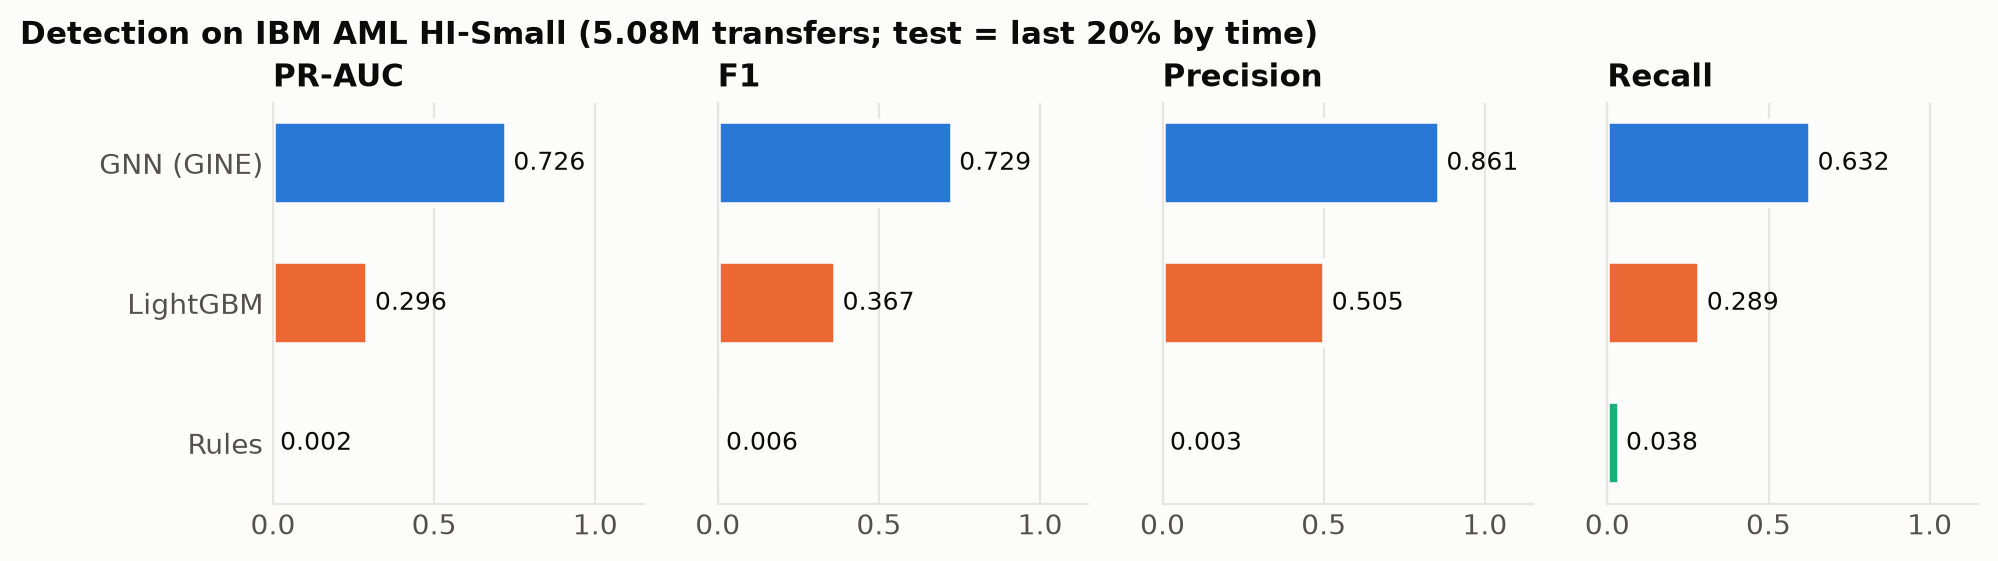
\includegraphics[width=\linewidth]{fig1_hi_small_detection.png}
\caption{Detection metrics on HI-Small (test = last 20\% by time)}
\label{fig:detection}
\end{figure}

\subsection{Robustness on the Digital Twin}
On the clean twin both detectors catch injected rings well (F1 0.974 for LightGBM, 0.971 for the GNN; ring recall 0.825 and 0.883). Table~\ref{tab:attacks} and Figure~\ref{fig:attacks} show the effect of each attack operator alone.

\begin{table}[H]
\centering
\renewcommand{\arraystretch}{1.2}
\setlength{\tabcolsep}{4pt}
{\small
\begin{tabular}{|l|c|c|c|c|c|c|c|c|}
\hline
 & \multicolumn{4}{c|}{\textbf{LightGBM}} & \multicolumn{4}{c|}{\textbf{GNN}} \\ \hline
\textbf{Attack} & \textbf{F1 att.} & \textbf{F1 retr.} & $\mathbf{D}$ & $\mathbf{R}$ & \textbf{F1 att.} & \textbf{F1 retr.} & $\mathbf{D}$ & $\mathbf{R}$ \\ \hline
camouflage & 0.493 & 0.823 & +0.481 & +0.330 & 0.535 & 0.848 & +0.436 & +0.313 \\ \hline
split & 0.535 & 0.976 & +0.439 & +0.441 & 0.933 & 0.986 & +0.038 & +0.053 \\ \hline
mimic & 0.667 & 0.961 & +0.307 & +0.294 & 0.869 & 0.965 & +0.102 & +0.096 \\ \hline
delay & 0.963 & 0.965 & +0.011 & +0.002 & 0.971 & 0.967 & +0.000 & $-$0.004 \\ \hline
add\_hops & 0.979 & 0.998 & $-$0.005 & +0.019 & 0.990 & 1.000 & $-$0.019 & +0.010 \\ \hline
separate\_owners & 0.974 & 0.974 & 0.000 & 0.000 & 0.971 & 0.969 & 0.000 & $-$0.002 \\ \hline
\end{tabular}}
\caption{Single-operator attacks on the twin: F1 under attack and after retraining, degradation $D$ and recovery $R$}
\label{tab:attacks}
\end{table}

\begin{figure}[H]
\centering
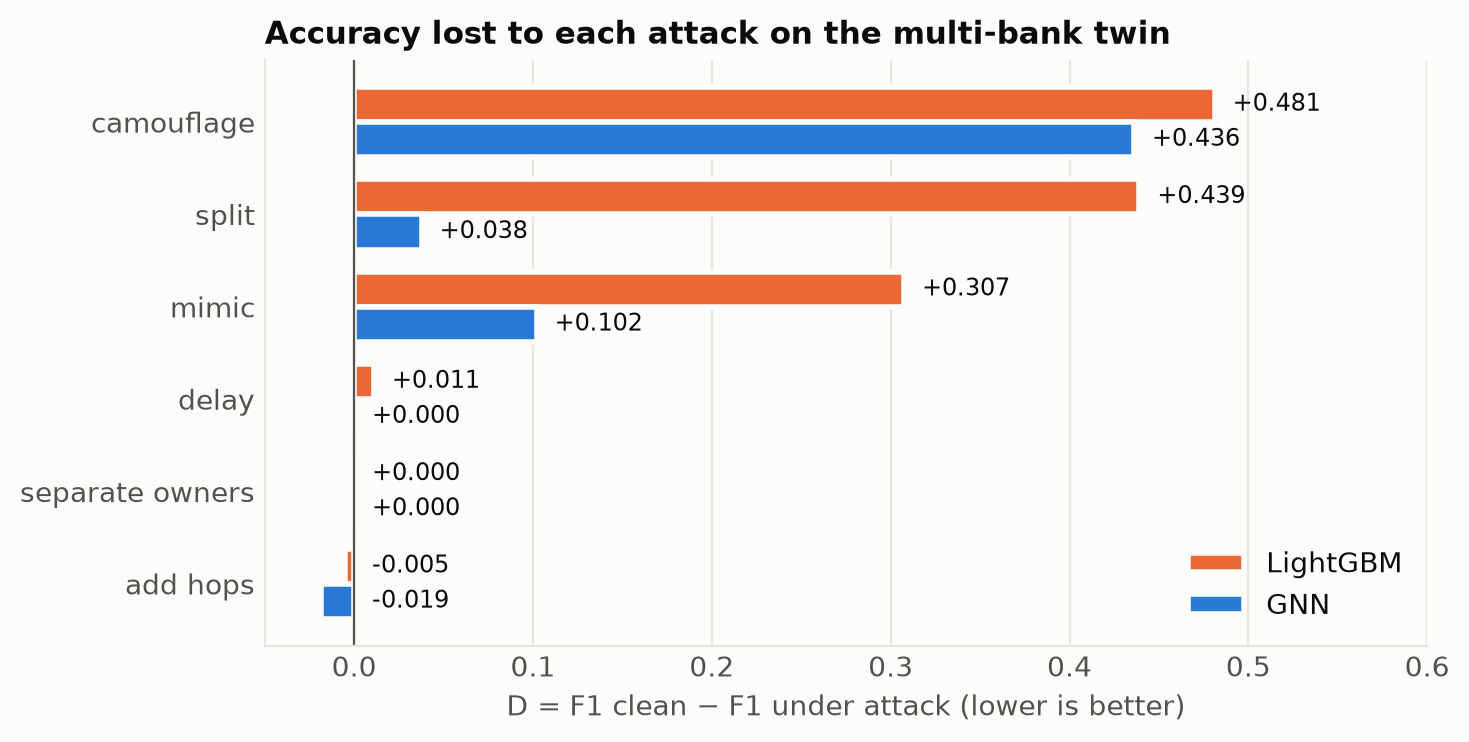
\includegraphics[width=0.88\linewidth]{fig2_attack_degradation.png}
\caption{Accuracy lost to each attack ($D$, lower is better)}
\label{fig:attacks}
\end{figure}

Three findings stand out. First, the graph view largely neutralises \textbf{structuring}: splitting transfers costs LightGBM 0.439 F1 but the GNN only 0.038, because the split transfers still connect the same accounts. Second, \textbf{feature mimicry} costs the GNN a third of what it costs LightGBM (0.102 versus 0.307): hiding the ACH cue removes a feature but not the structure. Third, \textbf{relation camouflage} --- mules padding their neighbourhoods with legitimate counterparties --- is the attack neither model shrugs off ($D$ = 0.481 and 0.436), and the only one that retraining repairs only partly (to 0.823 and 0.848). It attacks the aggregation step itself, as CARE-GNN predicted \cite{dou2020enhancing}.

Against the \textbf{adaptive attacker} (Table~\ref{tab:adaptive}, Figure~\ref{fig:adaptive}) the attacker chose a different first tactic for each model --- splitting against LightGBM and mimicry against the GNN --- confirming that it exploits the specific weakness of the deployed detector. After four rounds the GNN retains a retrained F1 of 0.878 against 0.834 for LightGBM.

\begin{table}[H]
\centering
\renewcommand{\arraystretch}{1.2}
\setlength{\tabcolsep}{4pt}
{\small
\begin{tabular}{|c|l|c|c|c|l|c|c|c|}
\hline
 & \multicolumn{4}{c|}{\textbf{LightGBM}} & \multicolumn{4}{c|}{\textbf{GNN}} \\ \hline
\textbf{Round} & \textbf{Added} & \textbf{F1 att.} & \textbf{F1 retr.} & $\mathbf{D}$ & \textbf{Added} & \textbf{F1 att.} & \textbf{F1 retr.} & $\mathbf{D}$ \\ \hline
1 & split & 0.535 & 0.976 & +0.439 & mimic & 0.869 & 0.965 & +0.102 \\ \hline
2 & mimic & 0.532 & 0.964 & +0.444 & split & 0.884 & 0.980 & +0.081 \\ \hline
3 & delay & 0.891 & 0.937 & +0.073 & camouflage & 0.634 & 0.897 & +0.346 \\ \hline
4 & camouflage & 0.586 & 0.834 & +0.351 & delay & 0.858 & 0.878 & +0.039 \\ \hline
\end{tabular}}
\caption{Adaptive multi-round attacker}
\label{tab:adaptive}
\end{table}

\begin{figure}[H]
\centering
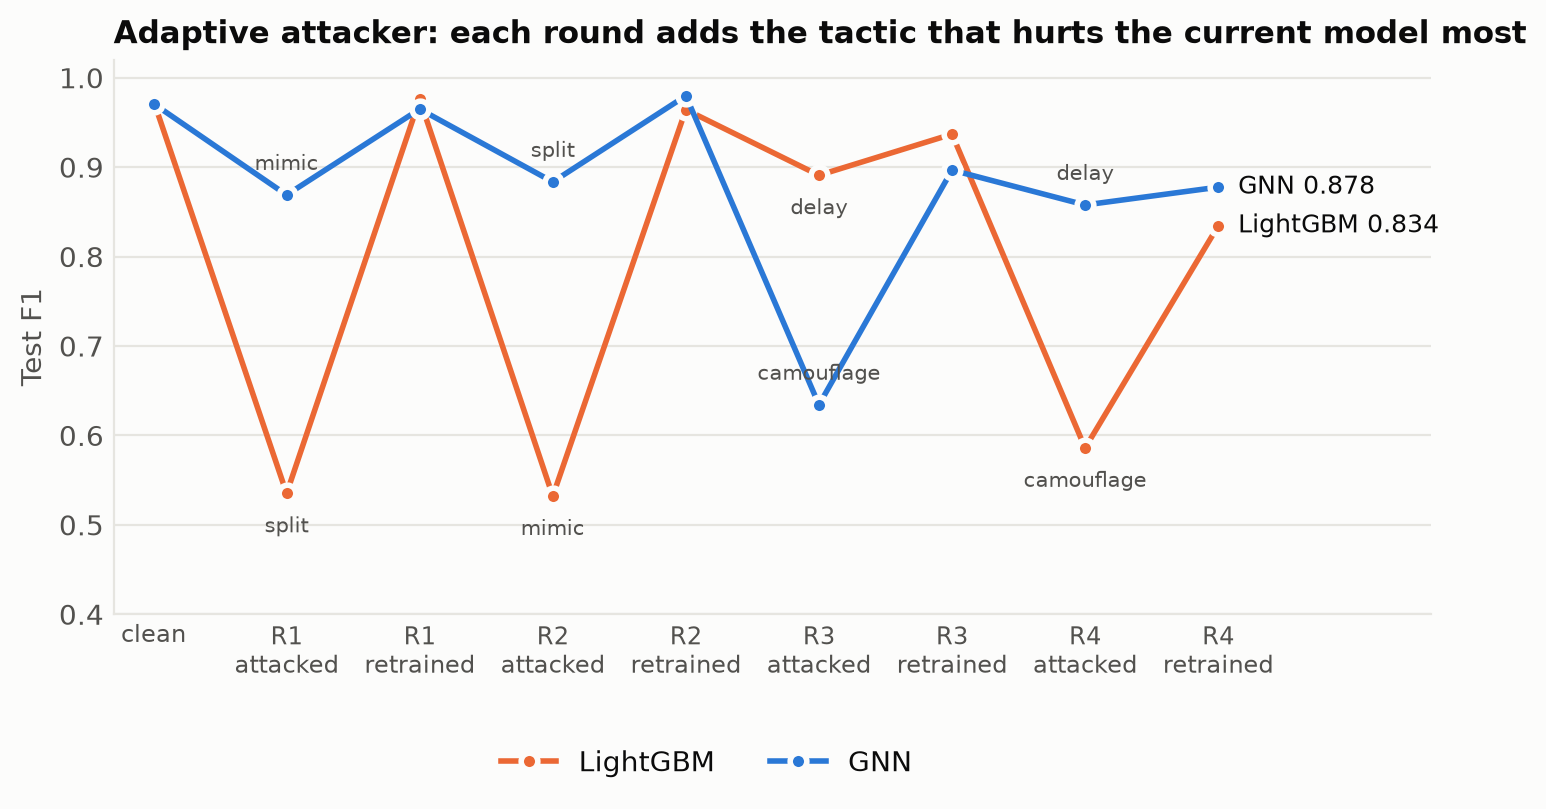
\includegraphics[width=0.92\linewidth]{fig3_adaptive_rounds.png}
\caption{Test F1 across four rounds of the adaptive attacker}
\label{fig:adaptive}
\end{figure}

\subsection{Investigation Agent}
For each of the 103 test-period rings, an investigation was opened at the ring's highest-scoring transfer and the reconstructed accounts were compared with the ground truth (Table~\ref{tab:agent}, Figure~\ref{fig:agent}). On the clean twin the agent recovers 98.9\% of ring accounts with 90.8\% precision and identifies the victim in 95.1\% of cases. Under camouflage, cover transactions pull legitimate counterparties into the reconstruction (precision 0.743) and the victim is found in 72.8\% of cases --- a quantitative reason why freezing must remain an officer's decision.

\begin{table}[H]
\centering
\renewcommand{\arraystretch}{1.25}
\begin{tabular}{|l|c|c|c|c|c|}
\hline
\textbf{Twin} & \textbf{Rings detected} & \textbf{Precision} & \textbf{Recall} & \textbf{Jaccard} & \textbf{Victim found} \\ \hline
clean & 103/103 & 0.908 & 0.989 & 0.899 & 0.951 \\ \hline
split attack & 103/103 & 0.891 & 0.992 & 0.885 & 0.961 \\ \hline
camouflage attack & 103/103 & 0.743 & 0.894 & 0.678 & 0.728 \\ \hline
\end{tabular}
\caption{Ring reconstruction by the investigation agent}
\label{tab:agent}
\end{table}

\begin{figure}[H]
\centering
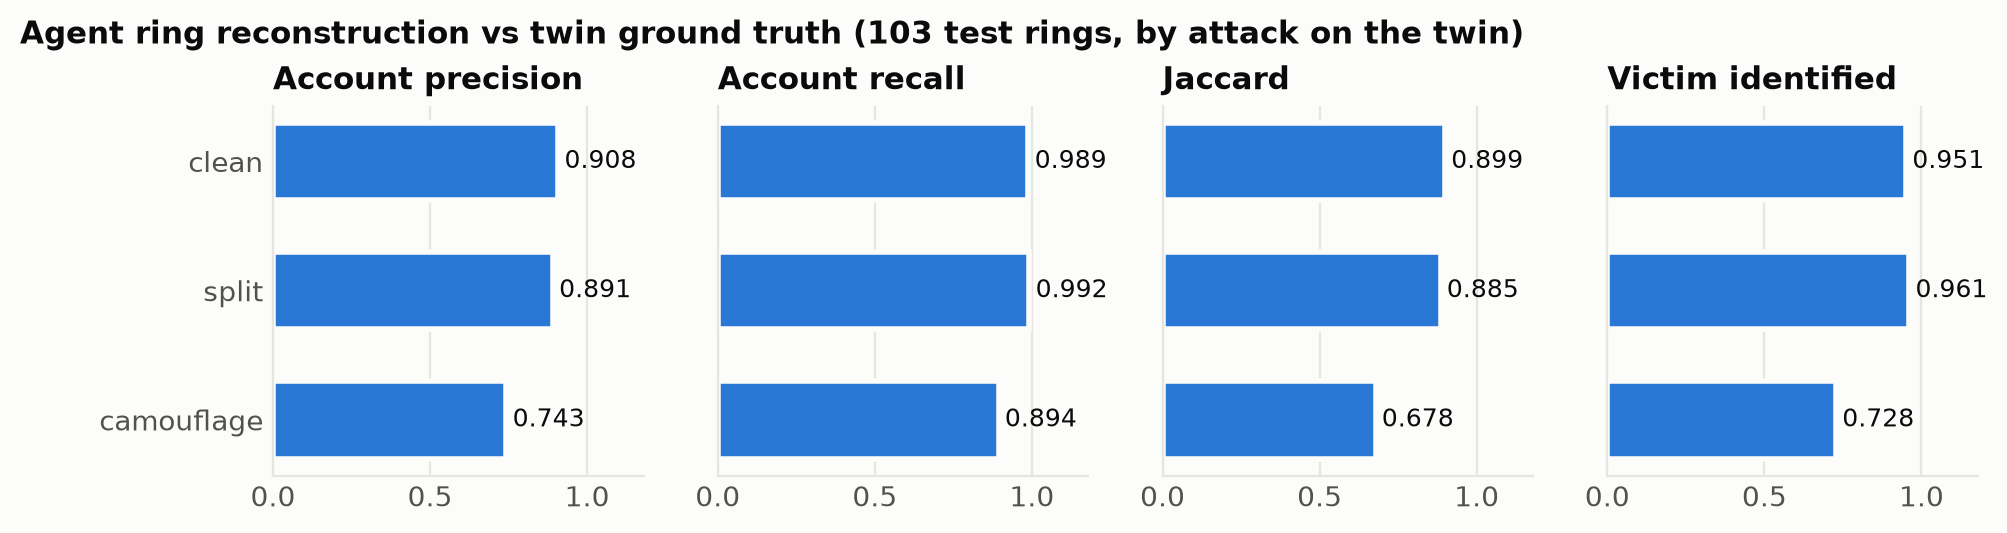
\includegraphics[width=\linewidth]{fig4_agent_reconstruction.png}
\caption{Agent ring reconstruction against twin ground truth}
\label{fig:agent}
\end{figure}

The language-model narrative was tested live on four cases. All four drafts were accepted after grounding, two after one repair. During development the check caught a genuine error: a draft stated ``eight dormant accounts'' where the case file recorded seven. Counts written in words were not checked at first; the count check was added because of this case.

\subsection{Discussion and Limitations}
The results support the two claims of the project: a heterogeneous temporal GNN detects cross-bank laundering far better than tabular models on the same features, and it is also markedly more robust to structuring and feature mimicry. Relation camouflage is the weakness that adversarial evaluation exposes and that retraining alone does not repair. The following limitations apply. The twin results come from a single random seed and should be repeated with several seeds before error bars are quoted. All data is synthetic; this is deliberate, since only synthetic data provides complete ground truth, but transfer to real bank data is not established. The full-data GNN was trained once, with the GINE backbone; GATv2 and GraphSAGE remain to be compared. The grounding check verifies numbers and counts, not every qualitative claim of the narrative.
